\section{Unvollständigkeit von RS-B2 in unterschiedlichen Szenarien}

In dieser Sektion wir die Unvollständigkeit von RS-B2, die nun auch experimentell gezeigt wurde, noch weiter ausgelotet. Zu diesem Zweck wurde der in Abb. \ref{Morphologischer} Kasten gebildet. Aus jeder Spalte des morphologischen Kastens werden Einträge gewählt und so Szenarien gebildet. Mit Hilfe dieser Szenarien, soll der Unvollständigkeit von RS-B2 weiter beleuchtet und Indizien für etwaige Bedingen der Unvollständigkeit gesammelt werden.


\begin{figure}[ht]
\centering
\resizebox{\textwidth}{!}{%
\begin{tabular}{|l|l|l|l|l|l|}
\hline
{\bf Algorithmus} & {\bf Anzahl an Knoten} & {\bf Formen} &  {\bf Initialer Baum} & {\bf Selektvität}    & {\bf Kardinalitäten} \\ \hline
RS-B0             & 5                      & Stern        & Bushy                 & Standard (0.5)       & Standard (10)        \\ \hline
RS-B1             & 7                      & Kette        & Links-tief             & Zufällig (0.0 - 1.0) & Zufällig (1 -100)    \\ \hline
RS-B2             & 9                    & Zyklisch         & Rechts-tief            &                      &                      \\ \hline
GraphRule         &                     &      &                       &                      &                      \\ \hline
\end{tabular}
}
\caption{Morphologischer Kasten zur Testgenerierung}
\label{Morphologischer}
\end{figure}


\subsection{Sternförmige Join-Graphen mit 5 Relationen}

In diesem Test werden die Regelmengen RS-B0, RS-B1 und RS-B2 im Kontext von sternförmigen Abfragen geprüft. Es werden unterschiedliche Formen der Bäume gewählt.

In den Abbildungen \ref{left-deep5-star.png} kann die Konfiguration abgelesen werden. Die anderen test unterscheiden sich in der Form, dass die Join-Trees entweder rechts-tief bzw. Bushy sind, soweit dies möglich ist. (Es wurde immer ein Knoten links als auch rechts an einen Basis Join angehängt.

\begin{figure}[ht]
  \centering
  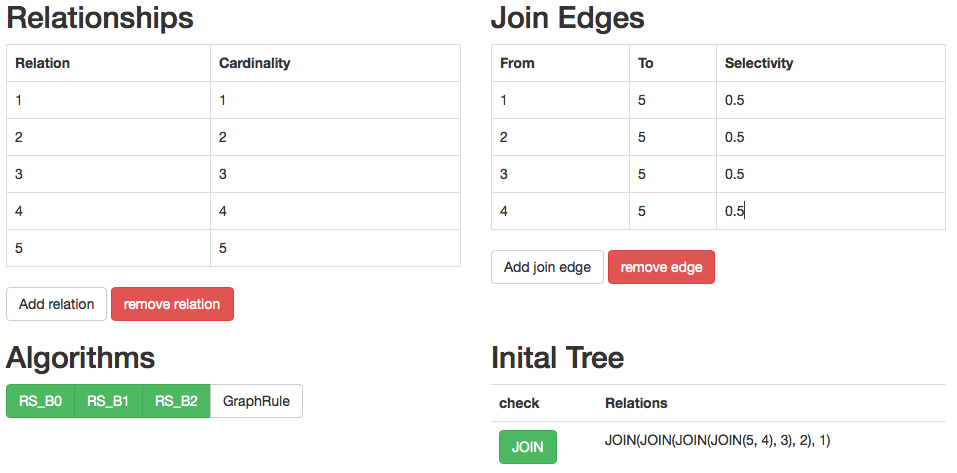
\includegraphics[width=\textwidth]{05_ResultsEvaluation/00_media/left-deep5-star.png}
  \caption{Konfiguration: Star-Join-Graph}
  \label{left-deep5-star.png}
\end{figure}





\begin{figure}[ht]
\centering
\resizebox{\textwidth}{!}{%
\begin{tabular}{|l|l|l|l|l|l|l|l|l|l|}
\hline
            & \multicolumn{3}{l|}{RS-B0}             & \multicolumn{3}{l|}{RS-B1}             & \multicolumn{3}{l|}{RS-B2}             \\ \hline
            & Äqui. & Pläne & ms & Äqui. & Pläne & ms & Äqui. & Pläne & ms \\ \hline
Links-Tief  & 39                & 384   & 75.894     & 39                & 384   & 71.184     & 39                & 384   & 65.211     \\ \hline
Bushy       & 39                & 384   & 75.768     & 39                & 384   & 72.485     & 39                & 384   & 66.498     \\ \hline
Rechts-Tief & 39                & 384   & 74.929     & 39                & 384   & 71.428     & 39                & 384   & 66.760     \\ \hline
\end{tabular}
}
\caption{Resultat: Star-Join-Graph}
\label{Star-Join-Graph:Result}
\end{figure}

In Abb. \ref{Star-Join-Graph:Result} sind die Ergebnisse der Test dargestellt. Es fällt auf, dass sowohl die Anzahld er Äquivalenzklassen (Äqui.) und die Anzahl der Pläne nicht unterscheiden. Die Dauer (gemessen in ms = Microsektunden) ist für alle initialen Pläne praktisch gleich. Nur minimale Abweichungen treten auf. Es kann davon asugegangen werden, dass alle Pläne gefunden wurden. Erstaunlich ist, dass die Ausführung von RS-B2 deutlich schneller war, als die der anderen Regelmengen. Es konnten jeweils ca. 10k - 15k ms eingespart werden.

\subsection{Kettenförmige Join-Graphen}

In dieser Testreihe soll bestimmt werden, ob alle Pläne aus einem kettenförmigen Join-Graphen gebildet werden können. Am Beispiel von links-tiefen Join-Graphen werden immer mehr Knoten angehängt und so die Geschwindigkeit und Vollständigkeit geprüft. Für den Vergleichstest aus RS-Graph, werden auch die Werte für RS-Graph angegeben.


\subsection{Zyklische Join-Graphen}
Tests wurden auch mit zyklischen Graphen durchgeführt. Zuerst wurde ein Test mit dem Join-Graphen durchgeführt, der in Abb. \ref{CylceJoin1} dargestellt wurde. In diesem Test konnte mir RS-B2 nicht jeder Plan generiert werden. Insgesamt wurden knapp 200 Pläne nicht generiert und so knapp 6 Äquivalenzklassen weniger erzeugt. 


\begin{figure}[ht]
  \centering
  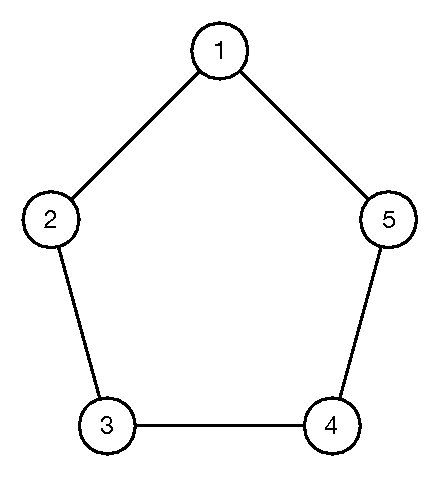
\includegraphics[scale=0.75]{05_ResultsEvaluation/00_media/CycleJoin1.pdf}
  \caption{Join-Graph: Zyklische Abfrage 1}
  \label{CylceJoin1}
\end{figure}






\begin{figure}[ht]
  \centering
  \begin{tabular}{|l|l|l|l|}
\hline
                  & RS-B0  & RS-B1  & RS-B2  \\ \hline
Äquivalenzklassen & 41     & 41     & 35     \\ \hline
Pläne             & 560    & 560    & 368    \\ \hline
Dauer (ms)        & 86.069 & 74.154 & 41.929 \\ \hline
\end{tabular}
  \caption{Resultat: Zyklische Abfrage 1}
  \label{ResCylceJoin1}

\end{figure}


Bei den Ergebnissen aus Abb. \ref{ResCylceJoin1} kann nun analysiert werden, welche Transformationen nicht stattgefunden haben. Hierzu wurden nur Transformationen betrachtet, die nicht durch Kommutativität direkt erzeugt wurden.

Je nach Anzahl der Relationen, die an der Transformation beteiligt waren, wurde eine unterschiedliche Anzahl an durchgeführten Transformationen festgestellt (vgl. Abb. \ref{involvedRelations}).


\begin{figure}[ht]
\centering

\begin{tabular}{|l|l|l|}
\hline
{\bf Relationen} & {\bf RS-B1} & {\bf RS-B2} \\ \hline
3                & 10          & 4           \\ \hline
4                & 30          & 6           \\ \hline
5                & 60          & 6           \\ \hline
\end{tabular}

\caption{Anzahl der Transformationen nach involvierten Relationen}
\label{involvedRelations}
\end{figure}


Bei einem Vergleich der durchgeführten Transformationen mit 3 Relationen fällt auf, warum RS-B2 nicht vollständig ist. In Abbildung \ref{Transformations3Rel} sind die Transformationen, die in den Regelmengen RS-B1 bzw. RS-B2 vorkommen mit x markiert. Transformationen, die nur Ergebnisse liefern, die mit Hilfe von Kommutativität in ihre Ursprungsform gebracht werden können, wurden mit o markiert, da diese Ergebnisse auch mit RS-B2 erzeugt werden können.


Zwei Transformationen wurden nicht markiert: $(45,1)-\textgreater(4,15)$ und $(15,4)-\textgreater(1,45)$. Sie werden nicht von RS-B2 erzeugt. Da jedoch das zweite Ergebnis auch mit Hilfe von Kommutativität aus dem ersten der beiden Startpläne erzeugt werden kann, muss es nicht weiter betrachtet werden.


\begin{figure}[ht]
\centering
\begin{tabular}{|l|l|l|}
\hline
{\bf Transformation}   & {\bf RS-B1} & {\bf RS-B2} \\ \hline
(12,3)-\textgreater(1,23) & x           & x           \\ \hline
(23,1)-\textgreater(3,12) & x           & o           \\ \hline
(23,4)-\textgreater(2,34) & x           & x           \\ \hline
(34,2)-\textgreater(4,23) & x           & o           \\ \hline
(12,5)-\textgreater(2,15) & x           & x           \\ \hline
(15,2)-\textgreater(5,12) & x           & o           \\ \hline
(34,5)-\textgreater(3,45) & x           & x           \\ \hline
(45,3)-\textgreater(5,34) & x           & o           \\ \hline
(45,1)-\textgreater(4,15) & x           &             \\ \hline
(15,4)-\textgreater(1,45) & x           &             \\ \hline
\end{tabular}


\caption{Transformationen mit 3 Relationen}
\label{Transformations3Rel}
\end{figure}

Es stellt sich die Frage, warum konnte diese Transformation nicht erreicht werden? Die Ursache findet sich im Join-Graphen \ref{CylceJoin1}. Die Knoten 4 und 5 sind unmittelbar miteinander verbunden. Der Knoten 1 jedoch nur über die Knoten 2 und 3. Um die Mittelbarkeit zu überwinden, musste zuerst Assoziativität angewendet werden.

Damit die Transformationen, die bei RS-B2 nicht durchgeführt wurden, möglich sind, muss eine Reihe von anderen Transformationen zuvor durchgeführt werden. 

Beispielsweise könnte nach einer Reihe von Transformationen die folgenden Graphen entstehen:

\begin{enumerate}
\item $((((1 \Join_{1} 2) \Join_{2} 3) \Join_{3} 4) \Join_{4} 5)$
\item $(1 \Join_{5} (2 \Join_{6} (3 \Join_{7} (4 \Join_{8} 5))))$
\item $(1 \Join_{5} ((2 \Join_{9} 3) \Join_{10} (4 \Join_{11} 5)))$
\item $((1 \Join_{5} (4 \Join_{11} 5)) \Join_{10} ((2 \Join_{9} 3)  ))$
\end{enumerate}

Im ersten Schritt wird ein links-tiefer Baum gebildet.
In einem zweiten Schritt muss die Relation 1 nach oben gezogen werden und der Teilbaum $4 \Join 5$ gebildet werden. Im dritten Schritt wird 4 und 5 auf eine Ebene mit 2 und 3 gebracht, um dann in Schritt 4 die Form $1 \Join (4 \Join 5)$ zu bilden.

Es fällt auf, dass i, die Form $1 \Join (4 \Join 5)$ zu erreichen auf alle Joins Transformationen angewendet werden mussten.


Wie bereits zuvor in Kapitel 3 besprochen, darf auf das Produkt einer Transformation nur Kommutativität angewendet werden. Daher ist es nicht möglich, eine Transformation der Form (15,4) -\textgreater (1,45) bzw. umgekehrt durchzuführen.


Klar ist, nicht nur das Beispiel aus Kapitel 3 zeigt die Unvollständigkeit von RS-B2. Auch bei zyklischen Graphen kann RS-B2 nicht alle alternativen Pläne erzeugen.


\subsection{Durchführung mit 4 Relationen}

Das Experiement wurde auch mit 4 Relationen durchgeführt. Auch hier gib es ein ähnliches Ergebnis (Abb. \ref{ResCylceJoin2}).

\begin{figure}[ht]
  \centering
  \begin{tabular}{|l|l|l|l|}
\hline
                  & RS-B0  & RS-B1  & RS-B2  \\ \hline
Äquivalenzklassen & 25     & 25     & 23     \\ \hline
Pläne             & 80    & 80    & 64    \\ \hline
Dauer (ms)        & 7.241 & 6.952 & 4.680 \\ \hline
\end{tabular}
  \caption{Resultat: Zyklische Abfrage 2}
  \label{ResCylceJoin2}

\end{figure}


Der Test wurde wie zuvor auch mit einem links-tiefen Baum durchgeführt. Wie bereits beschrieben, war es nicht möglich alle Pläne mit RS-B2 zu bilden. Strukturell ähnlich Transformationen konnten nicht durchgeführt werden.

\subsection{Vereinfachung des Beispiels aus Kapitel 3}

Nachdem nun festgestellt wurde, dass auch bei 4 Relationen in einem Zyklus nicht alle Pläne gefunden werden, wurde das Beispiel aus Abbildung 3.1 vereinfacht und erneut getestet. Dabei wurde die Frage gestellt: Ist es möglich mit dem Join-Graphen aus Abb. \ref{CylceJoin3} aus dem initialen Tree Q1 der neue Tree Q2 bilden?

\begin{figure}[ht]
  \centering
  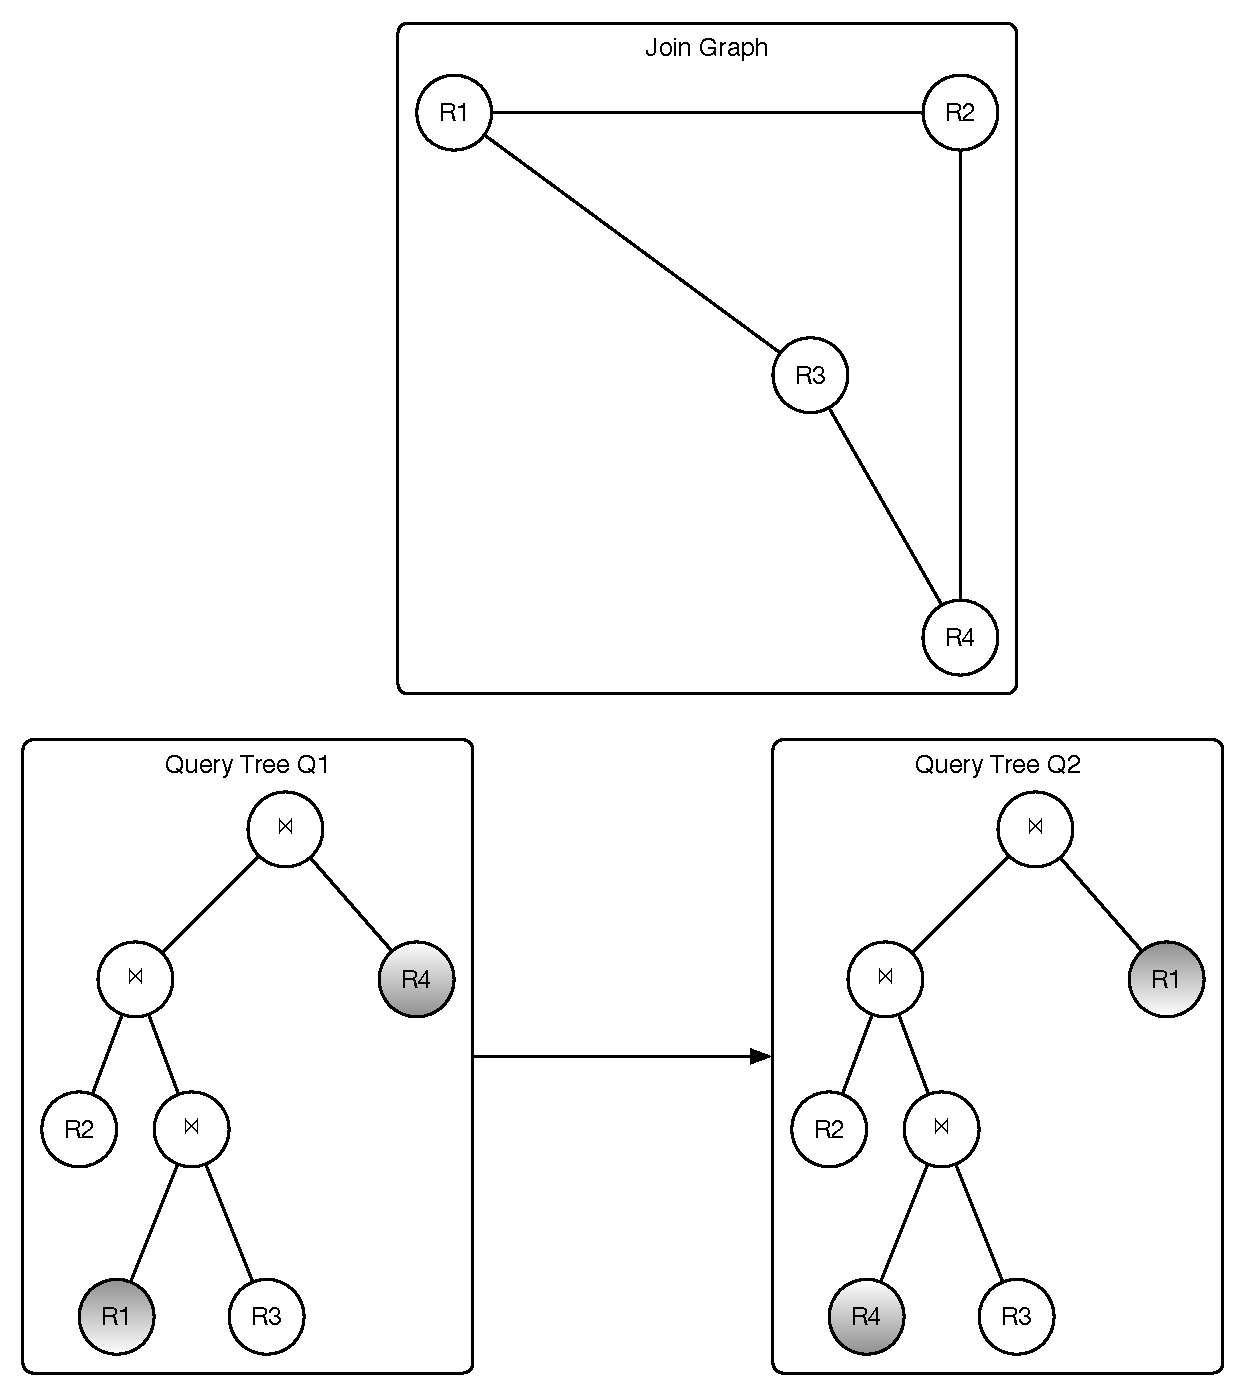
\includegraphics[scale=0.5]{05_ResultsEvaluation/00_media/CycleJoin3.pdf}
  \caption{Unvollständigkeit von RS-B2 vereinfacht}
  \label{CylceJoin3}
\end{figure}

Auch diese Transformation des Baums konnte zwar mit RS-B1 bzw. RS-B0 durchgeführt werden, jedoch nicht mit RS-B2.

\subsection{Fazit: Unvollständigkeit}
Die Experimente weisen darauf hin, dass RS-B2 bei zyklischen Join-Graphen unvollständig ist. Dies konnte in zwei Fällen gezeigt werden. Hingegen ist eine Unvollständigkeit bei sternförmigen bzw. kettenförmigen Join-Graphen nicht gefunden worden.